%!TEX root = ./main.tex

\section[Both at once]{Both Rulers from One Packet (SpotFi)}

% SECTION TIMING: 62:00--70:00 (2 frames). SpotFi's move: the CSI of ONE packet
% already contains both rulers -- 3 antennas (space) x 30 subcarriers (frequency).
% Fit angle AND delay per path jointly; the direct path is the earliest one; then
% cross bearings from the APs that can hear the phone.

% Teaching note (210 s): walk the four panels left to right. Collect CSI at every
% AP. Each path shows up as a pair (angle, delay). The direct path is the one with
% the smallest delay AND a stable bearing (ArrayTrack's trick, reused). Intersect the
% direct bearings. The trick that makes it work on THREE antennas: treat every
% (antenna, subcarrier) cell as a sensor -- 90 sensors per packet, not 3.
\begin{frame}{Angle and delay from the same packet}
  \vspace{0.3em}
  \centering
  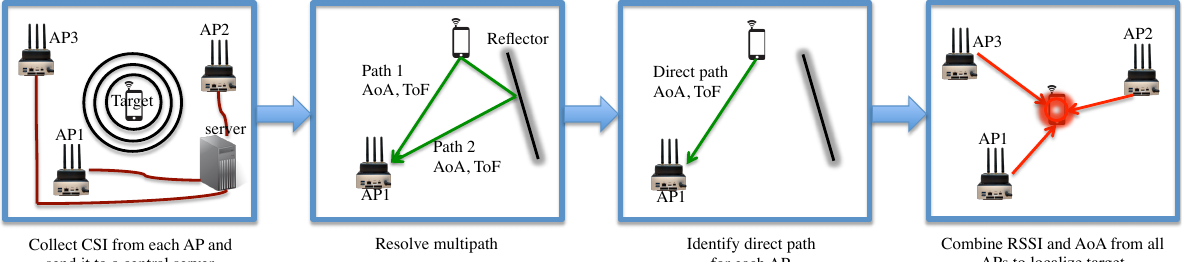
\includegraphics[width=0.98\textwidth]{figure/spotfi_overview.png}

  \vspace{0.5em}
  \raggedright
  {\small
   \begin{itemize}\itemsep3pt
     \item 3 antennas $\times$ 30 subcarriers $=$ \textbf{90 sensors} in one
       packet's CSI.
     \item Every path becomes an (\textcolor{ranblue}{angle},
       \textcolor{coreorange}{delay}) pair; fit them jointly.
     \item Direct path $=$ the \textbf{earliest} pair with a stable bearing.
       Then cross the bearings.
   \end{itemize}\par}
  \source{https://dl.acm.org/doi/10.1145/2785956.2787487}{Figure 1: Kotaru, Joshi, Bharadia \& Katti, SpotFi, SIGCOMM 2015}
\end{frame}

% Teaching note (120 s): same office, same three-antenna hardware: SpotFi 0.4 m
% median, ArrayTrack's algorithm 1.8 m. In the no-line-of-sight corridor SpotFi
% degrades to 1.6 m -- say that too. Close the loop: the question on slide one is
% answered with stock access points and nothing else.
\begin{frame}{A stock 3-antenna AP: 40 cm median}
  \vspace{0.3em}
  \centering
  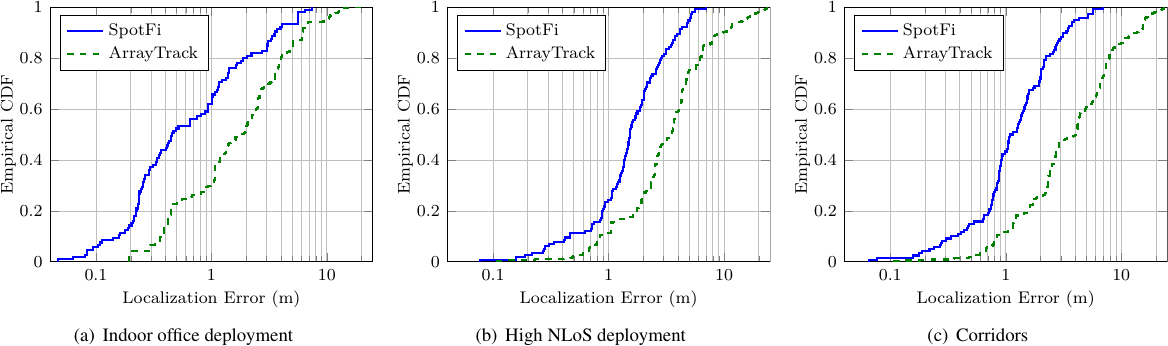
\includegraphics[width=0.98\textwidth]{figure/spotfi_cdf.png}

  \vspace{0.5em}
  {\small Same office, same 3-antenna hardware: SpotFi \textbf{0.4 m} median vs.\
   1.8 m for angle-only. Without line of sight: 1.6 m.\par}
  \vspace{0.4em}
  \takeaway{``Where is the phone?'' --- answered to 40 cm\\
    by access points that were already on the wall.}
  \source{https://dl.acm.org/doi/10.1145/2785956.2787487}{Figure 7: SpotFi, SIGCOMM 2015}
\end{frame}
